% Requires in the preamble:
% \usepackage{amsmath,amssymb}
% \usepackage{tikz,pgfplots}
% \pgfplotsset{compat=1.18}

\appendix
\chapter{Algebra and Inequalities Review}
\label{app:algebra-inequalities-review}

Calculus often fails in the algebra, not in the calculus.

A limit may look impossible until a factor cancels.  An integral may look unfamiliar
until a square is completed.  A derivative formula may be easier to read after radicals
are rewritten as powers.  A theorem may ask for an interval, and the interval may come
from solving an inequality carefully.

This appendix collects the algebra that appears again and again in the book.  It is not
meant to replace a full algebra course.  It is a repair bench.  When a calculation in the
main text gets stuck, the tool you need is often here.

\section{Factoring and completing the square}
\label{appsec:factoring-completing-square}

Factoring turns addition into multiplication.  That is why it is so useful in calculus.
Multiplication can cancel.  Multiplication has signs we can track.  Multiplication reveals
zeros.

\subsection{Common factors}
\label{appsubsec:common-factors}

The first question in factoring is always:

\[
\text{Is there a common factor?}
\]

For example,

\[
6x^3-9x^2=3x^2(2x-3).
\]

The common factor \(3x^2\) was present in both terms.

\paragraph{Example.}
Factor

\[
4x^4-8x^3+12x^2.
\]

Each term contains \(4x^2\), so

\[
4x^4-8x^3+12x^2
=
4x^2(x^2-2x+3).
\]

The quadratic \(x^2-2x+3\) does not factor over the real numbers, because its
discriminant is

\[
(-2)^2-4(1)(3)=4-12=-8<0.
\]

So the real factorization is

\[
\boxed{
4x^4-8x^3+12x^2=4x^2(x^2-2x+3).
}
\]

\subsection{Special products}
\label{appsubsec:special-products}

Some patterns appear often enough that they should become automatic.

\begin{center}
\renewcommand{\arraystretch}{1.6}
\begin{tabular}{c|c}
\textbf{name} & \textbf{identity} \\ \hline
Difference of squares &
\(\displaystyle a^2-b^2=(a-b)(a+b)\) \\

Perfect square &
\(\displaystyle a^2+2ab+b^2=(a+b)^2\) \\

Perfect square &
\(\displaystyle a^2-2ab+b^2=(a-b)^2\) \\

Difference of cubes &
\(\displaystyle a^3-b^3=(a-b)(a^2+ab+b^2)\) \\

Sum of cubes &
\(\displaystyle a^3+b^3=(a+b)(a^2-ab+b^2)\)
\end{tabular}
\end{center}

\paragraph{Example.}
Factor

\[
x^2-9.
\]

This is a difference of squares:

\[
x^2-9=x^2-3^2=(x-3)(x+3).
\]

\paragraph{Example.}
Factor

\[
4x^2+12x+9.
\]

This is a perfect square:

\[
4x^2+12x+9=(2x)^2+2(2x)(3)+3^2.
\]

Therefore

\[
\boxed{
4x^2+12x+9=(2x+3)^2.
}
\]

\subsection{Factoring quadratics}
\label{appsubsec:factoring-quadratics}

A quadratic has the form

\[
ax^2+bx+c.
\]

When \(a=1\), factoring asks for two numbers whose product is \(c\) and whose sum is
\(b\).

\paragraph{Example.}
Factor

\[
x^2+5x+6.
\]

We need two numbers with product \(6\) and sum \(5\).  They are \(2\) and \(3\).
Thus

\[
\boxed{
x^2+5x+6=(x+2)(x+3).
}
\]

\paragraph{Example.}
Factor

\[
x^2-x-12.
\]

We need two numbers with product \(-12\) and sum \(-1\).  They are \(-4\) and \(3\).
Thus

\[
\boxed{
x^2-x-12=(x-4)(x+3).
}
\]

When the leading coefficient is not \(1\), one reliable method is grouping.

\paragraph{Example.}
Factor

\[
6x^2+x-2.
\]

First multiply the leading coefficient and constant term:

\[
6(-2)=-12.
\]

We need two numbers with product \(-12\) and sum \(1\).  They are \(4\) and \(-3\).
Rewrite the middle term:

\[
6x^2+x-2=6x^2+4x-3x-2.
\]

Group:

\[
6x^2+4x-3x-2
=
2x(3x+2)-1(3x+2).
\]

Now factor out the common binomial:

\[
\boxed{
6x^2+x-2=(3x+2)(2x-1).
}
\]

\subsection{Why factoring matters in limits}
\label{appsubsec:factoring-limits}

A common calculus move is to simplify a difference quotient.

\paragraph{Example.}
Simplify

\[
\frac{(2+h)^2-4}{h},
\qquad h\neq0.
\]

Expand:

\[
(2+h)^2-4=4+4h+h^2-4=4h+h^2.
\]

Factor:

\[
4h+h^2=h(4+h).
\]

Therefore

\[
\frac{(2+h)^2-4}{h}
=
\frac{h(4+h)}{h}.
\]

Since \(h\neq0\),

\[
\boxed{
\frac{(2+h)^2-4}{h}=4+h.
}
\]

The cancellation is legal because \(h\neq0\).  That condition matters.  The original
fraction is undefined at \(h=0\), but the simplified expression \(4+h\) shows what the
fraction approaches as \(h\) gets close to \(0\).

\subsection{Completing the square}
\label{appsubsec:completing-square}

Factoring is not always possible.  Completing the square is often the next best move.

The pattern is

\[
x^2+bx
=
\left(x+\frac b2\right)^2-\left(\frac b2\right)^2.
\]

So

\[
\boxed{
x^2+bx+c
=
\left(x+\frac b2\right)^2+c-\left(\frac b2\right)^2.
}
\]

\paragraph{Example.}
Complete the square:

\[
x^2-6x+10.
\]

Half of \(-6\) is \(-3\).  Square it:

\[
(-3)^2=9.
\]

Add and subtract \(9\):

\[
x^2-6x+10
=
(x^2-6x+9)+1.
\]

Therefore

\[
\boxed{
x^2-6x+10=(x-3)^2+1.
}
\]

This form immediately tells us that

\[
x^2-6x+10\ge1
\]

for every real \(x\), because \((x-3)^2\ge0\).

\begin{figure}[h]
\centering
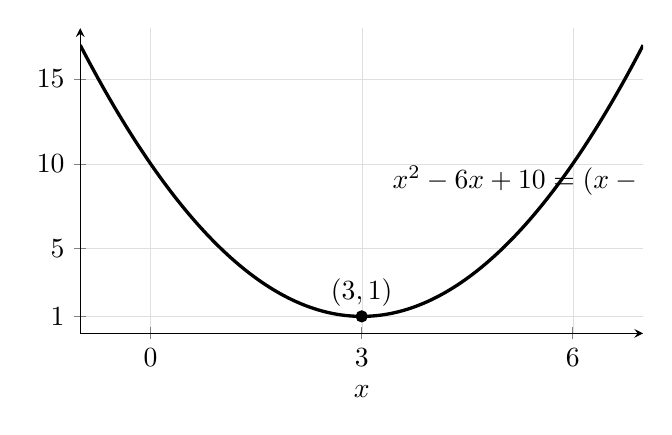
\begin{tikzpicture}
\begin{axis}[
    width=0.72\textwidth,
    height=0.45\textwidth,
    xmin=-1, xmax=7,
    ymin=0, ymax=18,
    axis lines=left,
    xlabel={\(x\)},
    ylabel={},
    xtick={0,3,6},
    ytick={1,5,10,15},
    grid=both,
    grid style={line width=.1pt, draw=gray!25},
]
\addplot[very thick, domain=-1:7, samples=150] {(x-3)^2+1};
\addplot[only marks, mark=*] coordinates {(3,1)};
\node[anchor=south] at (axis cs:3,1) {\((3,1)\)};
\node[anchor=west] at (axis cs:3.3,9) {\(x^2-6x+10=(x-3)^2+1\)};
\end{axis}
\end{tikzpicture}
\caption{Completing the square reveals the vertex and the minimum value.}
\label{fig:completing-square-vertex}
\end{figure}

\paragraph{Example.}
Complete the square for

\[
2x^2+8x-5.
\]

First factor out the leading coefficient from the quadratic and linear terms:

\[
2x^2+8x-5=2(x^2+4x)-5.
\]

Complete the square inside the parentheses.  Half of \(4\) is \(2\), and \(2^2=4\):

\[
x^2+4x=(x+2)^2-4.
\]

Thus

\[
2(x^2+4x)-5
=
2\bigl((x+2)^2-4\bigr)-5.
\]

So

\[
\boxed{
2x^2+8x-5=2(x+2)^2-13.
}
\]

This form tells us that the minimum value is \(-13\), reached at \(x=-2\).

\subsection{Quadratic formula}
\label{appsubsec:quadratic-formula}

Completing the square also gives the quadratic formula.  For

\[
ax^2+bx+c=0,
\qquad a\neq0,
\]

the solutions are

\[
\boxed{
x=\frac{-b\pm\sqrt{b^2-4ac}}{2a}.
}
\]

The expression

\[
b^2-4ac
\]

is called the \emph{discriminant}.  It tells how many real roots the quadratic has.

\begin{center}
\renewcommand{\arraystretch}{1.4}
\begin{tabular}{c|c}
\textbf{discriminant} & \textbf{real roots} \\ \hline
\(b^2-4ac>0\) & two distinct real roots \\
\(b^2-4ac=0\) & one repeated real root \\
\(b^2-4ac<0\) & no real roots
\end{tabular}
\end{center}

\paragraph{Example.}
Solve

\[
2x^2+8x-5=0.
\]

Here

\[
a=2,\qquad b=8,\qquad c=-5.
\]

So

\[
x=\frac{-8\pm\sqrt{8^2-4(2)(-5)}}{2(2)}
=
\frac{-8\pm\sqrt{64+40}}{4}.
\]

Thus

\[
x=\frac{-8\pm\sqrt{104}}4
=
\frac{-8\pm2\sqrt{26}}4.
\]

Therefore

\[
\boxed{
x=\frac{-4\pm\sqrt{26}}2.
}
\]

\section{Rational expressions}
\label{appsec:rational-expressions}

A rational expression is a quotient of polynomials, such as

\[
\frac{x^2-1}{x-1}.
\]

Rational expressions are common in limits, derivatives, partial fractions, and algebraic
simplification before integration.

The first rule is about domain:

\[
\boxed{
\text{A rational expression is undefined wherever its denominator is \(0\).}
}
\]

\subsection{Canceling common factors}
\label{appsubsec:canceling-common-factors}

Consider

\[
\frac{x^2-1}{x-1}.
\]

The numerator factors:

\[
x^2-1=(x-1)(x+1).
\]

So

\[
\frac{x^2-1}{x-1}
=
\frac{(x-1)(x+1)}{x-1}.
\]

For \(x\neq1\), we may cancel the common factor \(x-1\):

\[
\boxed{
\frac{x^2-1}{x-1}=x+1,
\qquad x\neq1.
}
\]

The condition \(x\neq1\) stays.  The original expression was not defined at \(x=1\).
Canceling a factor simplifies nearby values, but it does not restore the missing input.

\begin{quote}
\textbf{Cancel factors, not terms.}

This is legal:

\[
\frac{(x-1)(x+1)}{x-1}=x+1,
\qquad x\neq1.
\]

This is not legal:

\[
\frac{x^2-1}{x-1}\neq \frac{x^2}{x}=x.
\]

The numerator \(x^2-1\) is a difference, not a product.
\end{quote}

\paragraph{Example.}
Simplify

\[
\frac{x^2+5x+6}{x^2-9}.
\]

Factor numerator and denominator:

\[
x^2+5x+6=(x+2)(x+3),
\]

and

\[
x^2-9=(x-3)(x+3).
\]

Therefore

\[
\frac{x^2+5x+6}{x^2-9}
=
\frac{(x+2)(x+3)}{(x-3)(x+3)}.
\]

Cancel the common factor \(x+3\), but keep the domain restrictions:

\[
\boxed{
\frac{x^2+5x+6}{x^2-9}
=
\frac{x+2}{x-3},
\qquad x\neq -3,\;3.
}
\]

The simplified expression still must remember that \(x=-3\) and \(x=3\) were forbidden
in the original denominator.

\subsection{Combining rational expressions}
\label{appsubsec:combining-rational-expressions}

To add or subtract rational expressions, use a common denominator.

\paragraph{Example.}
Simplify

\[
\frac{2}{x}+\frac{3}{x+1}.
\]

The common denominator is \(x(x+1)\).  Thus

\[
\frac{2}{x}
=
\frac{2(x+1)}{x(x+1)},
\]

and

\[
\frac{3}{x+1}
=
\frac{3x}{x(x+1)}.
\]

So

\[
\frac{2}{x}+\frac{3}{x+1}
=
\frac{2(x+1)+3x}{x(x+1)}.
\]

Therefore

\[
\boxed{
\frac{2}{x}+\frac{3}{x+1}
=
\frac{5x+2}{x(x+1)},
\qquad x\neq0,-1.
}
\]

\paragraph{Example.}
Simplify the complex fraction

\[
\frac{\frac1x-\frac1a}{x-a},
\qquad x\neq0,\ a\neq0,\ x\neq a.
\]

First simplify the numerator:

\[
\frac1x-\frac1a
=
\frac{a-x}{ax}
=
-\frac{x-a}{ax}.
\]

Then

\[
\frac{\frac1x-\frac1a}{x-a}
=
\frac{-\frac{x-a}{ax}}{x-a}.
\]

Since \(x\neq a\), cancel \(x-a\):

\[
\boxed{
\frac{\frac1x-\frac1a}{x-a}
=
-\frac1{ax}.
}
\]

This kind of expression appears when differentiating \(1/x\) from the definition.

\subsection{Rationalizing}
\label{appsubsec:rationalizing}

Rationalizing means multiplying by a conjugate to remove a radical from a sum or
difference.

The basic identity is

\[
(A-B)(A+B)=A^2-B^2.
\]

\paragraph{Example.}
Simplify

\[
\frac{\sqrt{x+1}-1}{x},
\qquad x\neq0,\ x\ge -1.
\]

Multiply by the conjugate:

\[
\frac{\sqrt{x+1}-1}{x}
\cdot
\frac{\sqrt{x+1}+1}{\sqrt{x+1}+1}.
\]

The numerator becomes

\[
(\sqrt{x+1})^2-1^2=x+1-1=x.
\]

Thus

\[
\frac{\sqrt{x+1}-1}{x}
=
\frac{x}{x(\sqrt{x+1}+1)}.
\]

Since \(x\neq0\),

\[
\boxed{
\frac{\sqrt{x+1}-1}{x}
=
\frac{1}{\sqrt{x+1}+1}.
}
\]

This is exactly the algebra that makes the limit

\[
\lim_{x\to0}\frac{\sqrt{x+1}-1}{x}
\]

easy.

\section{Exponents and radicals}
\label{appsec:exponents-radicals}

Powers are the native language of many calculus formulas.  Radicals, roots, and
reciprocals are often easier to differentiate or integrate after they are rewritten as
powers.

\subsection{Laws of exponents}
\label{appsubsec:laws-exponents}

For positive bases, the usual exponent laws are:

\begin{center}
\renewcommand{\arraystretch}{1.7}
\begin{tabular}{c|c}
\textbf{law} & \textbf{example} \\ \hline
\(\displaystyle a^m a^n=a^{m+n}\) &
\(\displaystyle x^2x^5=x^7\) \\

\(\displaystyle \frac{a^m}{a^n}=a^{m-n}\) &
\(\displaystyle \frac{x^7}{x^3}=x^4\), \(x\neq0\) \\

\(\displaystyle (a^m)^n=a^{mn}\) &
\(\displaystyle (x^2)^5=x^{10}\) \\

\(\displaystyle (ab)^n=a^n b^n\) &
\(\displaystyle (3x)^2=9x^2\) \\

\(\displaystyle \left(\frac ab\right)^n=\frac{a^n}{b^n}\) &
\(\displaystyle \left(\frac{x}{2}\right)^3=\frac{x^3}{8}\), \(b\neq0\)
\end{tabular}
\end{center}

There are two common traps:

\[
(a+b)^2\neq a^2+b^2
\]

and

\[
\sqrt{a+b}\neq \sqrt a+\sqrt b.
\]

For example,

\[
(2+3)^2=25,
\]

but

\[
2^2+3^2=13.
\]

Also,

\[
\sqrt{9+16}=5,
\]

but

\[
\sqrt9+\sqrt{16}=7.
\]

\subsection{Negative and fractional exponents}
\label{appsubsec:negative-fractional-exponents}

A negative exponent means reciprocal:

\[
\boxed{
a^{-n}=\frac1{a^n},
\qquad a\neq0.
}
\]

A fractional exponent means a root:

\[
\boxed{
a^{1/n}=\sqrt[n]{a}
}
\]

when the root is defined.  More generally,

\[
\boxed{
a^{m/n}=\left(\sqrt[n]{a}\right)^m.
}
\]

For real-valued functions, even roots require nonnegative inputs:

\[
\sqrt{x}
\]

is real only for

\[
x\ge0.
\]

Odd roots allow all real inputs:

\[
\sqrt[3]{x}
\]

is real for every real \(x\).

\begin{center}
\renewcommand{\arraystretch}{1.6}
\begin{tabular}{c|c|c}
\textbf{expression} & \textbf{power form} & \textbf{domain as a real function} \\ \hline
\(\sqrt{x}\) & \(x^{1/2}\) & \(x\ge0\) \\
\(\sqrt[3]{x}\) & \(x^{1/3}\) & all real \(x\) \\
\(\displaystyle \frac1{x^2}\) & \(x^{-2}\) & \(x\neq0\) \\
\(\displaystyle \frac1{\sqrt{x}}\) & \(x^{-1/2}\) & \(x>0\) \\
\(\sqrt{x^2+1}\) & \((x^2+1)^{1/2}\) & all real \(x\)
\end{tabular}
\end{center}

\paragraph{Example.}
Rewrite using powers:

\[
\frac{3}{x^2\sqrt{x}}.
\]

Since

\[
\sqrt{x}=x^{1/2},
\]

we have

\[
x^2\sqrt{x}=x^2x^{1/2}=x^{5/2}.
\]

Therefore

\[
\boxed{
\frac{3}{x^2\sqrt{x}}=3x^{-5/2},
\qquad x>0.
}
\]

This form is easier to differentiate or integrate.

\paragraph{Example.}
Simplify

\[
(x^{3/2})(x^{5/2}).
\]

Add exponents:

\[
x^{3/2}x^{5/2}=x^{(3/2+5/2)}=x^{8/2}=x^4.
\]

So

\[
\boxed{
(x^{3/2})(x^{5/2})=x^4.
}
\]

\subsection{Radicals and conjugates}
\label{appsubsec:radicals-conjugates}

The conjugate of

\[
\sqrt{A}+\sqrt{B}
\]

is

\[
\sqrt{A}-\sqrt{B}.
\]

Multiplying gives

\[
(\sqrt{A}+\sqrt{B})(\sqrt{A}-\sqrt{B})=A-B.
\]

\paragraph{Example.}
Simplify

\[
\frac{1}{\sqrt{x+4}-2}.
\]

Multiply by the conjugate:

\[
\frac{1}{\sqrt{x+4}-2}
\cdot
\frac{\sqrt{x+4}+2}{\sqrt{x+4}+2}.
\]

The denominator becomes

\[
(x+4)-4=x.
\]

Therefore

\[
\boxed{
\frac{1}{\sqrt{x+4}-2}
=
\frac{\sqrt{x+4}+2}{x},
}
\]

where the original expression requires

\[
x\ge -4
\qquad\text{and}\qquad
x\neq0.
\]

The condition \(x\neq0\) appears because the original denominator is \(0\) when
\(\sqrt{x+4}=2\), which happens at \(x=0\).

\section{Inequalities and absolute values}
\label{appsec:inequalities-absolute-values}

Calculus uses inequalities to control error.

A limit proof says: make the input error small enough so that the output error is below
a chosen bound.  An approximation theorem says: the remainder is no larger than a
certain expression.  A convergence test says: compare one quantity with another.

So inequalities are not only algebraic chores.  They are the grammar of control.

\subsection{Rules for inequalities}
\label{appsubsec:rules-inequalities}

The safe rules are:

\begin{center}
\renewcommand{\arraystretch}{1.7}
\begin{tabular}{c|c}
\textbf{operation} & \textbf{rule} \\ \hline
Add the same number & If \(a<b\), then \(a+c<b+c\). \\

Subtract the same number & If \(a<b\), then \(a-c<b-c\). \\

Multiply by a positive number & If \(a<b\) and \(c>0\), then \(ac<bc\). \\

Multiply by a negative number & If \(a<b\) and \(c<0\), then \(ac>bc\). \\

Take reciprocals of positives & If \(0<a<b\), then \(\dfrac1a>\dfrac1b\).
\end{tabular}
\end{center}

The most common mistake is forgetting to reverse the inequality when multiplying or
dividing by a negative number.

\paragraph{Example.}
Solve

\[
-3x+5<11.
\]

Subtract \(5\):

\[
-3x<6.
\]

Divide by \(-3\).  Because \(-3\) is negative, reverse the inequality:

\[
\boxed{
x>-2.
}
\]

\subsection{Sign charts}
\label{appsubsec:sign-charts-inequalities}

For polynomial and rational inequalities, factoring and sign charts are usually safer
than expanding.

\paragraph{Example.}
Solve

\[
x^2-x-6>0.
\]

Factor:

\[
x^2-x-6=(x-3)(x+2).
\]

The critical numbers are

\[
x=-2
\qquad\text{and}\qquad
x=3.
\]

They split the real line into three intervals:

\[
(-\infty,-2),
\qquad
(-2,3),
\qquad
(3,\infty).
\]

Test one point in each interval.

\begin{center}
\renewcommand{\arraystretch}{1.4}
\begin{tabular}{c|c|c|c}
\textbf{interval} & \(x+2\) & \(x-3\) & \((x+2)(x-3)\) \\ \hline
\((-\infty,-2)\) & \(-\) & \(-\) & \(+\) \\
\((-2,3)\) & \(+\) & \(-\) & \(-\) \\
\((3,\infty)\) & \(+\) & \(+\) & \(+\)
\end{tabular}
\end{center}

We need the product to be positive, so

\[
\boxed{
x<-2
\quad\text{or}\quad
x>3.
}
\]

In interval notation,

\[
\boxed{
(-\infty,-2)\cup(3,\infty).
}
\]

Because the inequality is strict, the endpoints are not included.

\paragraph{Example.}
Solve

\[
\frac{x+1}{x-2}\le0.
\]

The numerator is zero at \(x=-1\).  The denominator is zero at \(x=2\), where the
expression is undefined.

These numbers split the line into

\[
(-\infty,-1),
\qquad
(-1,2),
\qquad
(2,\infty).
\]

\begin{center}
\renewcommand{\arraystretch}{1.4}
\begin{tabular}{c|c|c|c}
\textbf{interval} & \(x+1\) & \(x-2\) & \(\dfrac{x+1}{x-2}\) \\ \hline
\((-\infty,-1)\) & \(-\) & \(-\) & \(+\) \\
\((-1,2)\) & \(+\) & \(-\) & \(-\) \\
\((2,\infty)\) & \(+\) & \(+\) & \(+\)
\end{tabular}
\end{center}

We need the expression to be less than or equal to \(0\).  It is negative on
\((-1,2)\), and it is zero at \(x=-1\).  It is undefined at \(x=2\).

Therefore

\[
\boxed{
[-1,2).
}
\]

\subsection{Absolute value as distance}
\label{appsubsec:absolute-value-distance-review}

The absolute value \(|x|\) is the distance from \(x\) to \(0\).  More generally,

\[
\boxed{
|x-a|
}
\]

is the distance from \(x\) to \(a\).

This gives the most important translations:

\[
\boxed{
|x-a|<r
\quad\Longleftrightarrow\quad
a-r<x<a+r,
}
\qquad r>0,
\]

and

\[
\boxed{
|x-a|\le r
\quad\Longleftrightarrow\quad
a-r\le x\le a+r.
}
\]

\begin{figure}[h]
\centering
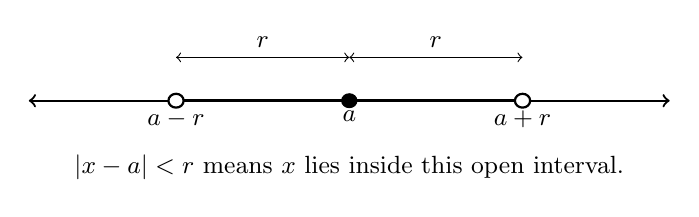
\begin{tikzpicture}[xscale=1.1, every node/.style={font=\small}]
  \draw[<->, thick] (-0.7,0) -- (6.7,0);

  \coordinate (L) at (1,0);
  \coordinate (A) at (3,0);
  \coordinate (R) at (5,0);

  \draw[very thick] (L) -- (R);
  \draw[fill=white, thick] (L) circle (2.5pt);
  \draw[fill=black] (A) circle (2.5pt);
  \draw[fill=white, thick] (R) circle (2.5pt);

  \node[below] at (L) {\(a-r\)};
  \node[below] at (A) {\(a\)};
  \node[below] at (R) {\(a+r\)};

  \draw[<->] (1,0.55) -- (3,0.55);
  \draw[<->] (3,0.55) -- (5,0.55);
  \node[above] at (2,0.55) {\(r\)};
  \node[above] at (4,0.55) {\(r\)};

  \node at (3,-0.85) {\(|x-a|<r\) means \(x\) lies inside this open interval.};
\end{tikzpicture}
\caption{Absolute value inequalities are distance statements.}
\label{fig:absolute-value-distance-appendix}
\end{figure}

\paragraph{Example.}
Solve

\[
|x-4|<0.2.
\]

This means that \(x\) is within \(0.2\) of \(4\).  Therefore

\[
4-0.2<x<4+0.2.
\]

So

\[
\boxed{
3.8<x<4.2.
}
\]

\paragraph{Example.}
Solve

\[
|2x+1|\le5.
\]

Translate to a compound inequality:

\[
-5\le2x+1\le5.
\]

Subtract \(1\):

\[
-6\le2x\le4.
\]

Divide by \(2\):

\[
\boxed{
-3\le x\le2.
}
\]

\subsection{Absolute value and limits}
\label{appsubsec:absolute-value-limits}

The notation in limits uses absolute value because limits are about distance.

For example,

\[
|x-2|<0.01
\]

means that \(x\) is within \(0.01\) of \(2\).

If

\[
f(x)=3x+1,
\]

then the distance from \(f(x)\) to \(7\) is

\[
|f(x)-7|
=
|3x+1-7|
=
|3x-6|
=
3|x-2|.
\]

So if we want

\[
|f(x)-7|<0.03,
\]

it is enough to require

\[
3|x-2|<0.03.
\]

That is,

\[
|x-2|<0.01.
\]

This is the algebraic heart of a simple epsilon-delta proof.  The absolute value measures
the input error and the output error.

\section{Sigma notation practice}
\label{appsec:sigma-notation-practice}

A long sum such as

\[
1^2+2^2+3^2+\cdots+n^2
\]

needs compact notation.  Sigma notation supplies it:

\[
\sum_{k=1}^n k^2.
\]

The Greek letter \(\Sigma\) means ``sum.''

\subsection{Reading sigma notation}
\label{appsubsec:reading-sigma}

The expression

\[
\sum_{k=1}^n a_k
\]

means

\[
a_1+a_2+\cdots+a_n.
\]

The index \(k\) starts at \(1\), increases by \(1\) each time, and stops at \(n\).

\paragraph{Example.}
Expand

\[
\sum_{k=1}^4 k^2.
\]

We substitute \(k=1,2,3,4\):

\[
\sum_{k=1}^4 k^2
=
1^2+2^2+3^2+4^2.
\]

Thus

\[
\sum_{k=1}^4 k^2
=
1+4+9+16=30.
\]

\paragraph{Example.}
Expand

\[
\sum_{j=0}^3 (2j+1).
\]

Substitute \(j=0,1,2,3\):

\[
\sum_{j=0}^3 (2j+1)
=
1+3+5+7=16.
\]

The letter \(j\) is temporary.  We could write

\[
\sum_{k=0}^3 (2k+1)
\]

and get the same number.

\begin{quote}
\textbf{Dummy index.}
The index of summation is a placeholder.  These mean the same thing:

\[
\sum_{k=1}^n k^2
=
\sum_{j=1}^n j^2
=
\sum_{m=1}^n m^2.
\]
\end{quote}

\subsection{Linearity of finite sums}
\label{appsubsec:linearity-finite-sums}

Sums behave well with addition and constant multiples:

\[
\boxed{
\sum_{k=1}^n (a_k+b_k)
=
\sum_{k=1}^n a_k+\sum_{k=1}^n b_k
}
\]

and

\[
\boxed{
\sum_{k=1}^n c\,a_k
=
c\sum_{k=1}^n a_k.
}
\]

These are finite versions of the linearity rules for integrals.

\paragraph{Example.}
Compute

\[
\sum_{k=1}^5 (3k-2).
\]

Use linearity:

\[
\sum_{k=1}^5 (3k-2)
=
3\sum_{k=1}^5 k-\sum_{k=1}^5 2.
\]

Now

\[
\sum_{k=1}^5 k=1+2+3+4+5=15
\]

and

\[
\sum_{k=1}^5 2=2+2+2+2+2=10.
\]

So

\[
\boxed{
\sum_{k=1}^5 (3k-2)=3(15)-10=35.
}
\]

\subsection{Basic sum formulas}
\label{appsubsec:basic-sum-formulas}

The most common finite sum formulas are:

\begin{center}
\renewcommand{\arraystretch}{1.8}
\begin{tabular}{c|c}
\textbf{sum} & \textbf{formula} \\ \hline
Constant sum &
\(\displaystyle \sum_{k=1}^n c=cn\) \\

First powers &
\(\displaystyle \sum_{k=1}^n k=\frac{n(n+1)}2\) \\

Squares &
\(\displaystyle \sum_{k=1}^n k^2=\frac{n(n+1)(2n+1)}6\) \\

Cubes &
\(\displaystyle \sum_{k=1}^n k^3=\left(\frac{n(n+1)}2\right)^2\) \\

Geometric sum &
\(\displaystyle \sum_{k=0}^{n} r^k=\frac{1-r^{n+1}}{1-r},\quad r\neq1\)
\end{tabular}
\end{center}

\paragraph{Example.}
Compute

\[
\sum_{k=1}^{10} k^2.
\]

Use the square formula:

\[
\sum_{k=1}^{10}k^2
=
\frac{10(11)(21)}6.
\]

Simplify:

\[
\frac{10(11)(21)}6
=
5(11)(7)
=
385.
\]

So

\[
\boxed{
\sum_{k=1}^{10} k^2=385.
}
\]

\paragraph{Example.}
Compute

\[
\sum_{k=0}^{4} 3^k.
\]

This is a geometric sum with \(r=3\):

\[
\sum_{k=0}^{4}3^k
=
\frac{1-3^5}{1-3}.
\]

So

\[
\sum_{k=0}^{4}3^k
=
\frac{1-243}{-2}
=
121.
\]

Checking by expansion:

\[
1+3+9+27+81=121.
\]

\subsection{Changing the index}
\label{appsubsec:changing-index}

Sometimes it helps to shift the index.

\paragraph{Example.}
Rewrite

\[
\sum_{k=3}^{n} k^2
\]

as a sum starting at \(1\).

Since

\[
\sum_{k=1}^{n} k^2
=
1^2+2^2+\sum_{k=3}^{n} k^2,
\]

we have

\[
\boxed{
\sum_{k=3}^{n} k^2
=
\sum_{k=1}^{n} k^2-1^2-2^2
=
\sum_{k=1}^{n} k^2-5.
}
\]

\paragraph{Example.}
Rewrite

\[
\sum_{k=0}^{n-1} \left(\frac{2k}{n}\right)^2
\]

using \(j=k+1\).

If

\[
j=k+1,
\]

then

\[
k=j-1.
\]

When \(k=0\), \(j=1\).  When \(k=n-1\), \(j=n\).  Therefore

\[
\sum_{k=0}^{n-1} \left(\frac{2k}{n}\right)^2
=
\sum_{j=1}^{n} \left(\frac{2(j-1)}{n}\right)^2.
\]

The two sums are the same.  Only the label changed.

\subsection{Sigma notation and Riemann sums}
\label{appsubsec:sigma-riemann-sums}

Sigma notation becomes essential when defining integrals.

For example, divide \([0,2]\) into \(n\) equal pieces.  Then

\[
\Delta x=\frac{2}{n}.
\]

Using right endpoints for \(f(x)=x^2\), the sample points are

\[
x_k=\frac{2k}{n},
\qquad k=1,2,\ldots,n.
\]

The right Riemann sum is

\[
\sum_{k=1}^{n} f(x_k)\Delta x
=
\sum_{k=1}^{n}
\left(\frac{2k}{n}\right)^2\frac{2}{n}.
\]

Simplify:

\[
\sum_{k=1}^{n}
\left(\frac{2k}{n}\right)^2\frac{2}{n}
=
\sum_{k=1}^{n}
\frac{8k^2}{n^3}.
\]

Pull out the constant:

\[
\frac{8}{n^3}\sum_{k=1}^{n}k^2.
\]

Use the square formula:

\[
\frac{8}{n^3}\cdot\frac{n(n+1)(2n+1)}6.
\]

So

\[
\boxed{
\sum_{k=1}^{n}
\left(\frac{2k}{n}\right)^2\frac{2}{n}
=
\frac{4(n+1)(2n+1)}{3n^2}.
}
\]

As \(n\to\infty\),

\[
\frac{4(n+1)(2n+1)}{3n^2}
\to
\frac{8}{3}.
\]

Thus the rectangle sums approach

\[
\int_0^2 x^2\,dx=\frac83.
\]

The sigma notation is not decoration.  It is the bridge from finite sums to integrals.

\section{Practice problems}
\label{appsec:algebra-practice-problems}

\subsection*{Factoring and completing the square}

\begin{enumerate}
\item Factor \(x^2+7x+12\).

\item Factor \(2x^2-5x-3\).

\item Factor \(x^3-8\).

\item Complete the square:
\[
x^2+10x+13.
\]

\item Complete the square:
\[
3x^2-12x+7.
\]

\item Solve:
\[
x^2-4x-5=0.
\]
\end{enumerate}

\subsection*{Rational expressions}

\begin{enumerate}
\item Simplify:
\[
\frac{x^2-4}{x-2}.
\]
State the restriction.

\item Simplify:
\[
\frac{x^2+3x+2}{x^2-1}.
\]
State the restrictions.

\item Simplify:
\[
\frac{1}{x}+\frac{1}{x+2}.
\]

\item Simplify:
\[
\frac{\frac1{x+h}-\frac1x}{h},
\qquad h\neq0.
\]

\item Rationalize:
\[
\frac{\sqrt{x+9}-3}{x}.
\]
\end{enumerate}

\subsection*{Exponents and radicals}

\begin{enumerate}
\item Rewrite as a power of \(x\):
\[
\frac{1}{x^3\sqrt{x}}.
\]

\item Simplify:
\[
x^{2/3}x^{5/3}.
\]

\item Rewrite using radicals:
\[
x^{3/2}.
\]

\item Simplify:
\[
\left(x^{-2}\right)^3.
\]

\item State the real domain of
\[
\frac{1}{\sqrt{x-4}}.
\]
\end{enumerate}

\subsection*{Inequalities and absolute values}

\begin{enumerate}
\item Solve:
\[
5-2x\le 11.
\]

\item Solve:
\[
x^2+x-6<0.
\]

\item Solve:
\[
\frac{x-4}{x+1}>0.
\]

\item Solve:
\[
|x-3|<0.5.
\]

\item Solve:
\[
|4x-1|\ge 7.
\]
\end{enumerate}

\subsection*{Sigma notation}

\begin{enumerate}
\item Expand:
\[
\sum_{k=1}^{5}(k^2+1).
\]

\item Compute:
\[
\sum_{k=1}^{20} k.
\]

\item Compute:
\[
\sum_{k=1}^{6} k^2.
\]

\item Compute:
\[
\sum_{k=0}^{5} 2^k.
\]

\item Write the right Riemann sum for \(f(x)=x^3\) on \([0,1]\) using \(n\) equal
subintervals.

\item Simplify the sum from the previous problem as much as possible using a sum
formula.
\end{enumerate}

\section*{Answers to Appendix A practice problems}
\label{ans:appendix-a-practice}

\subsection*{Factoring and completing the square}

\begin{enumerate}
\item
\[
x^2+7x+12=(x+3)(x+4).
\]

\item
\[
2x^2-5x-3=(2x+1)(x-3).
\]

\item
\[
x^3-8=(x-2)(x^2+2x+4).
\]

\item
\[
x^2+10x+13=(x+5)^2-12.
\]

\item
\[
3x^2-12x+7=3(x-2)^2-5.
\]

\item
\[
x^2-4x-5=(x-5)(x+1),
\]
so
\[
x=5
\qquad\text{or}\qquad
x=-1.
\]
\end{enumerate}

\subsection*{Rational expressions}

\begin{enumerate}
\item
\[
\frac{x^2-4}{x-2}
=
\frac{(x-2)(x+2)}{x-2}
=
x+2,
\qquad x\neq2.
\]

\item
\[
\frac{x^2+3x+2}{x^2-1}
=
\frac{(x+1)(x+2)}{(x-1)(x+1)}
=
\frac{x+2}{x-1},
\qquad x\neq -1,1.
\]

\item
\[
\frac{1}{x}+\frac{1}{x+2}
=
\frac{x+2+x}{x(x+2)}
=
\frac{2x+2}{x(x+2)}
=
\frac{2(x+1)}{x(x+2)}.
\]

\item
\[
\frac{\frac1{x+h}-\frac1x}{h}
=
\frac{\frac{x-(x+h)}{x(x+h)}}{h}
=
\frac{-h}{x(x+h)h}
=
-\frac1{x(x+h)}.
\]

\item
\[
\frac{\sqrt{x+9}-3}{x}
\cdot
\frac{\sqrt{x+9}+3}{\sqrt{x+9}+3}
=
\frac{x}{x(\sqrt{x+9}+3)}
=
\frac1{\sqrt{x+9}+3},
\]
with the original restrictions \(x\ge -9\) and \(x\neq0\).
\end{enumerate}

\subsection*{Exponents and radicals}

\begin{enumerate}
\item
\[
\frac{1}{x^3\sqrt{x}}=x^{-7/2}.
\]

\item
\[
x^{2/3}x^{5/3}=x^{7/3}.
\]

\item
\[
x^{3/2}=x\sqrt{x}.
\]

\item
\[
(x^{-2})^3=x^{-6}=\frac1{x^6}.
\]

\item
\[
\frac1{\sqrt{x-4}}
\]
requires
\[
x-4>0,
\]
so the domain is
\[
(4,\infty).
\]
\end{enumerate}

\subsection*{Inequalities and absolute values}

\begin{enumerate}
\item
\[
5-2x\le11
\]
gives
\[
-2x\le6.
\]
Divide by \(-2\) and reverse the inequality:
\[
x\ge -3.
\]

\item
\[
x^2+x-6=(x+3)(x-2).
\]
The product is negative between the roots, so
\[
-3<x<2.
\]

\item
The critical numbers are \(-1\) and \(4\).  The quotient is positive when numerator and
denominator have the same sign, so
\[
(-\infty,-1)\cup(4,\infty).
\]

\item
\[
|x-3|<0.5
\]
means
\[
2.5<x<3.5.
\]

\item
\[
|4x-1|\ge7
\]
means
\[
4x-1\le -7
\qquad\text{or}\qquad
4x-1\ge7.
\]
Thus
\[
x\le -\frac32
\qquad\text{or}\qquad
x\ge2.
\]
\end{enumerate}

\subsection*{Sigma notation}

\begin{enumerate}
\item
\[
\sum_{k=1}^{5}(k^2+1)
=
(1^2+1)+(2^2+1)+(3^2+1)+(4^2+1)+(5^2+1).
\]

\item
\[
\sum_{k=1}^{20}k=\frac{20(21)}2=210.
\]

\item
\[
\sum_{k=1}^{6}k^2=\frac{6(7)(13)}6=91.
\]

\item
\[
\sum_{k=0}^{5}2^k=\frac{1-2^6}{1-2}=63.
\]

\item
On \([0,1]\),

\[
\Delta x=\frac1n,
\qquad
x_k=\frac{k}{n}.
\]

The right Riemann sum is

\[
\sum_{k=1}^{n}\left(\frac{k}{n}\right)^3\frac1n.
\]

\item
\[
\sum_{k=1}^{n}\left(\frac{k}{n}\right)^3\frac1n
=
\frac1{n^4}\sum_{k=1}^{n}k^3.
\]

Using

\[
\sum_{k=1}^{n}k^3=\left(\frac{n(n+1)}2\right)^2,
\]

we get

\[
\frac1{n^4}\left(\frac{n(n+1)}2\right)^2
=
\frac{(n+1)^2}{4n^2}.
\]
\end{enumerate}